\documentclass[10pt,a4paper,printanswers]{upmc} 

\usepackage[T1]{fontenc}
\usepackage[utf8]{inputenc}
%\usepackage[english]{babel}
\usepackage{amsmath}
\usepackage{amssymb}
\usepackage[ruled,vlined,linesnumbered]{algorithm2e}
\usepackage{mathtools}
\usepackage[usenames,dvipsnames]{xcolor}
\usepackage{framed}
\usepackage[framemethod=tikz]{mdframed}
\usepackage{listings}         

\global\mdfdefinestyle{graybox}{%
  linecolor=black,linewidth=1pt,%
  backgroundcolor=lightgray
}

\mdfdefinestyle{evaluation}{
    frametitlebackgroundcolor=black!15,
    frametitlerule=true,
    roundcorner=10pt,
    middlelinewidth=1pt,
    innermargin=0.5cm,
    outermargin=0.5cm,
    innerleftmargin=0.5cm,
    innerrightmargin=0.5cm,
    innertopmargin=\topskip,
    innerbottommargin=\topskip,
    frametitle={Evaluation}
}

\usepackage[textwidth=18cm,textheight=25cm]{geometry}

\newcommand{\myline}{\noindent\makebox[\linewidth]{\rule{\textwidth}{0.7pt}}}
\newcommand{\mytilde}{\raise.17ex\hbox{$\scriptstyle\mathtt{\sim}$}}

\newcounter{mainmemorder}
\newcommand{\save}{\setcounter{mainmemorder}{\value{enumi}}}
\newcommand{\load}{\setcounter{enumi}{\value{mainmemorder}}}
\newcommand{\mytext}[1]{\colorbox{lightgray}{\texttt{#1}}}
\newcommand{\subsecline}{\texorpdfstring{\hrulefill}{}}

\newcommand{\Num}{Part 1}
\newcommand{\UE}{\scriptsize M1 ISI/SAR/IPS\\ ROS \& experimental robotics}

\title{ROS and experimental robotics.\\ How-to operate the Turtlebot 3 burger.}

\lstset{language=matlab,
  basicstyle=\small\sffamily,
  keywordstyle=\color{dblue}\bfseries,  
  commentstyle=\color{dred}\textit,
  stringstyle=\color{dgreen}\ttfamily,
  extendedchars=true,
  frame=single, 
  numbers=left,
  backgroundcolor=\color{lgray}
}

\begin{document}

\maketitle

Working with a real robot is not different from listening and subscribing to topics, using services,
etc.\ , except that the node you are working with is currently running on a distance
machine inside the robot.\\

To allow the ROS nodes running on the virtual machine to communicate with the nodes running
on the robot, the connections between the two must be first set up. To do that, ROS uses shell
variables that are declared in the file \texttt{.bashrc} at the root of the \texttt{turtle}
(virtual machine) and \texttt{ubuntu} (robot) user's home directory. Both must be modified as follows.

\begin{enumerate}
  \item Both the virtual machine and the robot must be on the same network. The robot automatically
        creates its own wifi hotspot (the name of this hotspot is \texttt{turblebot\_n} where n is
        the number of your turtlebot). This hotspot is accessible with the password
        \texttt{@turtlebot\_wifi@}. Connect your host machine (i.e. the computer on which is running
        the virtualization platform) to one of these wifi network (the one created by your robot).
  \item It is then necessary to modify the network configuration of the virtual machine, by
        switching from a "NAT shared" to a "Bridged" network (see Figure \ref{fig:bridged}), so that
        the virtual machine is on the same network as the turtlebot.
        \begin{figure}[!h]
          \centering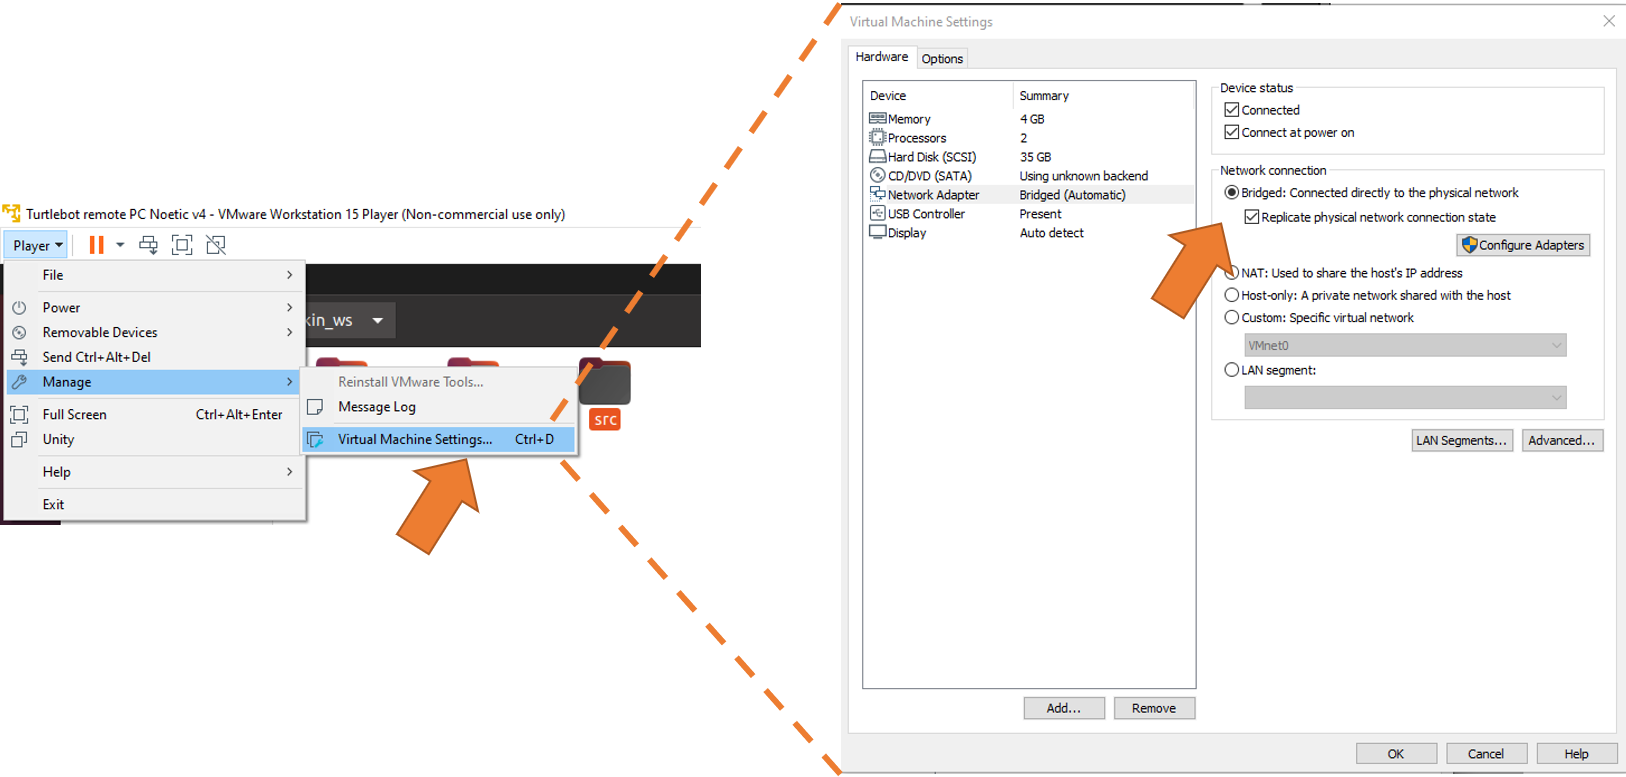
\includegraphics[height=6cm]{figures/bridged.png}
          \caption{Ubuntu window with the network connection details.}
          \label{fig:bridged}
        \end{figure}

  \item The robot should now get its IP address from the robot. To check it is the case, click on
        the arrow on the top right of the menu bar in Ubuntu, and click on the arrow next to
        \texttt{wired Connected} and then on \texttt{Wired Settings}. A window then appears, like in
        Figure~\ref{fig:wifi}. From there, note the IP address in the IPv4 section.
        %
        \begin{figure}[!h]
          \centering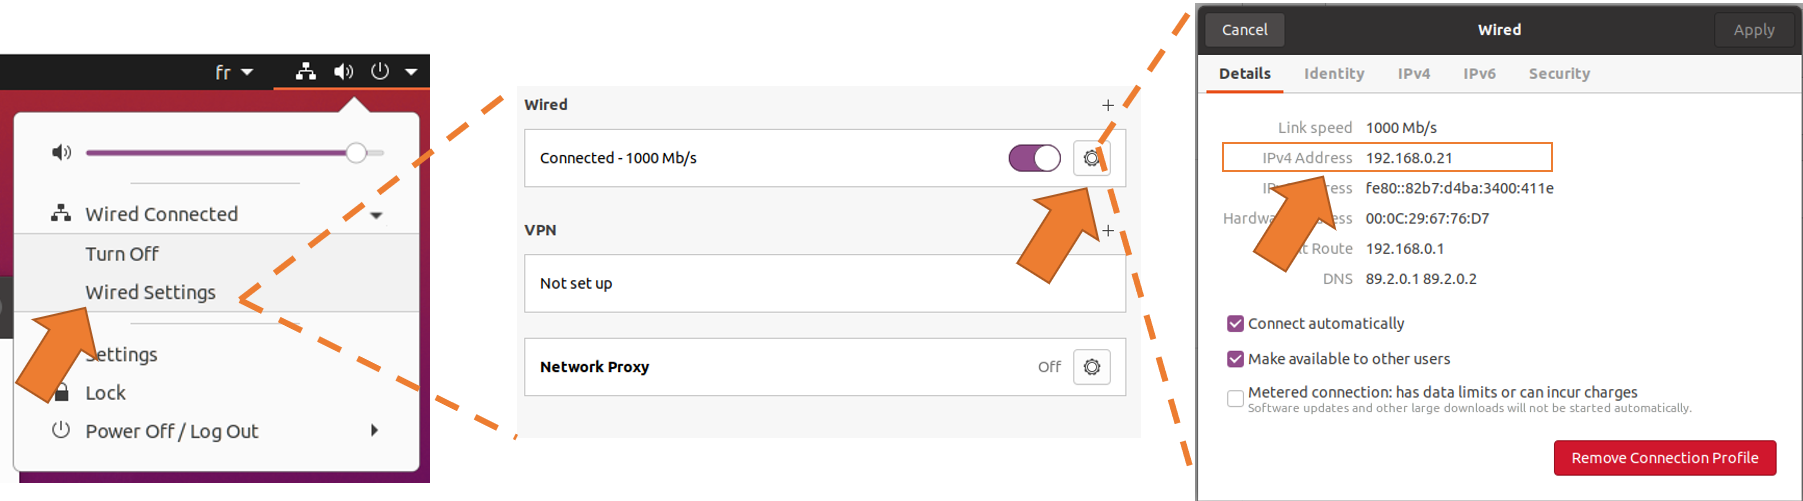
\includegraphics[height=4cm]{figures/wifi.png}
          \caption{Ubuntu window with the network connection details.}
          \label{fig:wifi}
        \end{figure}
        %
        \begin{mdframed}[style=graybox]
          You might have to perform this step every time you disconnect and reconnect to the wifi
          network, since the IP address you get from the robot might change. Only the IP address of
          each robot is fixed. If the VM IP address does not start with \texttt{192.168.0.} then try
          to reboot the virtual machine and start over.
        \end{mdframed}

  \item Edit the file \texttt{\mytilde/.bashrc} \textbf{in the virtual machine }by using the
        following command in a terminal
        \lstinputlisting[
          language=bash, % Use Perl functions/syntax highlighting
          frame=single, % Frame around the code listing
          showstringspaces=false, % Don't put marks in string spaces
          numbers=left, % Line numbers on left
          numberstyle=\tiny, % Line numbers styling
          basicstyle=\footnotesize,
        ]{code/gedit.shell}
        %
        A new window appears: scroll to the bottom of the file, and modify the to variables
        \texttt{ROS\_MASTER\_URI} and \texttt{ROS\_HOSTNAME} to include the IP address you get from
        the previous step. For instance, if the IP adress is \texttt{192.168.0.237}, the two lines
        must be then modified along: \lstinputlisting[
          language=bash, % Use Perl functions/syntax highlighting
          frame=single, % Frame around the code listing
          showstringspaces=false, % Don't put marks in string spaces
          numbers=left, % Line numbers on left
          numberstyle=\tiny, % Line numbers styling
          basicstyle=\footnotesize,
        ]{code/bashrc.shell}
        Do not forget to save your changes!

  \item The same must be done on the robot, except you have to remotely connect to it first. This
        time, getting the IP address of your robot is easy: it is written on a sticker placed near
        the laser at the top of the robot. For instance, lets consider the robot IP is
        \texttt{192.168.0.113}.

        Next, connect to the distant robot \textbf{from you virtual machine} by typing the following command in a terminal (if asked, the password is turtlebot):
        \lstinputlisting[
          language=bash, % Use Perl functions/syntax highlighting
          frame=single, % Frame around the code listing
          showstringspaces=false, % Don't put marks in string spaces
          numbers=left, % Line numbers on left
          numberstyle=\tiny, % Line numbers styling
          basicstyle=\footnotesize,
        ]{code/ssh.shell}
        %
        Then, you are \textbf{connected to the robot on a distant shell} in you terminal. From
        there, edit the \texttt{.bashrc} \textbf{on the robot} file using the following command:
        \lstinputlisting[
          language=bash, % Use Perl functions/syntax highlighting
          frame=single, % Frame around the code listing
          showstringspaces=false, % Don't put marks in string spaces
          numbers=left, % Line numbers on left
          numberstyle=\tiny, % Line numbers styling
          basicstyle=\footnotesize,
        ]{code/nano.shell}
        %
        A text editor is now opened in you terminal. Scroll down to the bottom of the opened file and
        modify here the two \texttt{ROS\_MASTER\_URI} and \texttt{ROS\_HOSTNAME} so that the former matches
        \textbf{the virtual machine IP} and the later \textbf{the robot IP}. For instance, the two lines
        must be modified along:
        \lstinputlisting[
          language=bash, % Use Perl functions/syntax highlighting
          frame=single, % Frame around the code listing
          showstringspaces=false, % Don't put marks in string spaces
          numbers=left, % Line numbers on left
          numberstyle=\tiny, % Line numbers styling
          basicstyle=\footnotesize,
        ]{code/bashrc_robot.shell}
        %
        Do not forget to save your changes by pressing \mytext{Ctrl+O} and next \mytext{Enter}, and quit
        the text editor with \mytext{Ctrl+X}. Thanks to these modifications, all running ROS nodes will
        communicate with the master running on your local virtual machine.
        %
  \item Now close all your running terminal to be sure your changes to be applied. Then, run the
        \mytext{roscore} command from a terminal on your local machine and log again on the robot using the
        \texttt{ssh} command shown before. On the robot, launch the \mytext{turtlebot3\_core.launch} file
        from the \mytext{turtlebot3\_bringup} packet. Check if the running nodes on the robot are correctly
        reaching the master on the local machine by checking if the IP address in the output messages
        matches the IP of the virtual machine.
        \begin{solution}
          \texttt{\$ roslaunch turtlebot3\_bringup turtlebot3\_core.launch}
        \end{solution}

  \item  You should now be able to teleoperate the turtlebot! Please call your teacher before actually trying to control the robot. This one must be first secured, and ideally placed above a small box so that both wheels can freely rotate without making the robot actually move.
        \begin{solution}
          \texttt{\$rosnode list}\\
          \texttt{\$rostopic list}\\
          The command must be sent to the topic \mytext{/cmd\_vel}.
        \end{solution}

\end{enumerate}

\end{document}
